\documentclass[11pt]{article}
%%%%%%%%% options for the file macros.tex

\def\showauthornotes{1}
\def\showkeys{0}
\def\showdraftbox{0}
\let\pref=\prettyref


\usepackage{amsmath, ulem, amssymb, amsfonts, hyperref, amsthm, listings, tcolorbox, bbm, xifthen, soul, mathtools}
\usepackage[margin=1in]{geometry}
\usepackage[linesnumbered,lined,boxed,commentsnumbered, ruled]{algorithm2e}
\hypersetup{
    colorlinks=true,
    linkcolor=blue,
    filecolor=magenta,      
    citecolor=magenta,      
    urlcolor=cyan,
}
\usepackage[
    backend=biber,
    style=alphabetic,
    sorting=ynt,
    backref=true
]{biblatex}
\usepackage[shortlabels]{enumitem}
\usepackage{cleveref}

\newtheorem{theorem}{Theorem}[section]
\newtheorem{lemma}[theorem]{Lemma}
\newtheorem{corollary}[theorem]{Corollary}
\newtheorem{claim}[theorem]{Claim}
\newtheorem{fact}[theorem]{Fact}
\newtheorem{open-problem}[theorem]{Open Problem}

\theoremstyle{definition}

\newtheorem{definition}[theorem]{Definition}
\newtheorem{example}[theorem]{Example}

\newtheorem{remark}{Remark}
\newtheorem{question}{Question}

\newcommand{\V}[1]{\mathbf{#1}\ignorespaces}
\renewcommand\AA{\boldsymbol{\mathit{A}}}
\newcommand\LL{\boldsymbol{\mathit{L}}}
\newcommand\MM{\boldsymbol{\mathit{M}}}
\newcommand\II{\boldsymbol{\mathit{I}}}
\newcommand\JJ{\boldsymbol{\mathit{J}}}
\newcommand\KK{\boldsymbol{\mathit{K}}}

\newcommand{\ab}[1]{\langle #1 \rangle}
\renewcommand{\subset}{\subseteq}
\newcommand{\dsquare}{\mathbin{\raisebox{.2ex}{
    \hspace{-.4em}$\bigcirc$\hspace{-.75em}{\rm s}\hspace{.15em}}}}
\newcommand{\from}{\overset{R}{\leftarrow}}
\newcommand{\1}{\mathbbm{1}}

\DeclareMathOperator{\USTCON}{USTCON}
\DeclareMathOperator{\STCON}{STCON}
\usepackage{graphicx}
\usepackage{epstopdf}

% For indenting algorithm pseudocode.
\algdef{SE}[SUBALG]{Indent}{EndIndent}{}{\algorithmicend\ }%
\algtext*{Indent}
\algtext*{EndIndent}

%%%%%%%%% Authornotes
\newcommand{\Snote}{\Authornote{S}}
\newcommand{\Scomment}{\Authorcomment{S}}
\newcommand{\Sfnote}{\Authorfnote{S}}

%%%%%%%%%%%%%%%%%%%%%%%%%

\begin{document}

\newcommand{\coursenum}{{CSC 2421H}}
\newcommand{\coursename}{{Graphs Matrices and Optimization}}
\newcommand{\courseprof}{Sushant Sachdeva}

\newenvironment{tight_enumerate}{
\begin{enumerate}
  \setlength{\itemsep}{2pt}
  \setlength{\parskip}{1pt}
}{\end{enumerate}}

\noindent
\begin{center}
\framebox{ \vbox{ \hbox to \textwidth { {\bf \coursenum\ :\
       \coursename} \hfill Lecture 8 : 12 Nov 2018}
   \vspace{3mm}
   \hbox to \textwidth { {\Large \hfill Graph Sparsifiers \hfill} }
   \vspace{1mm}
   \hbox to \textwidth { {\it Lecturer: \courseprof \hfill Scribe: Kevan Hollbach} }
 }
}
\end{center}
\vspace*{4mm}

\newtheorem{thm}{Theorem}
\newcommand{\LE}{\preceq}
\newcommand{\GE}{\succeq}
\newcommand{\bb}{\mathbb}
\newcommand{\E}{\mathbb{E}}
%\newcommand{\pr}{\text{Pr}} % already defined
%\newcommand{\eps}{\epsilon} % already defined
\newcommand{\mm}{\mu_{\min}}
\newcommand{\mM}{\mu_{\max}}
\newcommand{\lm}{\lambda_{\min}}
\newcommand{\lM}{\lambda_{\max}}
%\newcommand{\ones}{\textbf{1}} % already defined
\newcommand{\T}{\top}
\newcommand{\half}{{\frac{1}{2}}}
\newcommand{\mhalf}{{-\frac{1}{2}}}
\newcommand{\phalf}{{+/2}}
\newcommand{\Reff}{{R_{\textit{eff}}}}
\newcommand{\brac}[1]{\left[#1\right]}

\noindent
Recall the following theorem from last class.

\begin{theorem}
\label{thm:chernoff}
Let $0 < \eps < 1$, and let $\V{X}_1,\dots,\V{X}_t \in \bb{R}^{n \times n}$ be
symmetric independant random matrices such that
$\forall i \,:\, 0 \LE \V{X}_i \LE R \, \bb{I}$.
If $\mm \bb{I} \LE \E \sum \V{X}_i \LE \mM \bb{I}$
then
\begin{align*}
\Pr\brac{\sum \V{X}_i \GE (1 + \eps)\mM} &\le n \exp\paren{-\frac{\eps^2 \mM}{3R}} \text{ and} \\
\Pr\brac{\sum \V{X}_i \LE (1 - \eps)\mm} &\le n \exp\paren{-\frac{\eps^2 \mm}{2R}}.
\end{align*}
\end{theorem}

\noindent
In particular, this holds for $\mm = \lm(\E \sum \V{X}_i)$ and
$\mM = \lM(\E \sum \V{X}_i)$, the tightest bounds on the spectrum of the
expected sum.

\section{Spectral Graph Sparsifiers}

We introduce the notion of spectral sparsifiers, which are a generalization of
spectral expanders. Given a graph $G = (V,E)$, a graph $H = (V,E')$ is an
$\eps$-spectral sparsifier of $G$ if \[(1-\eps)\V{L}_G \LE \V{L}_H \LE (1+\eps)\V{L}_G.\]
In this case we will write $H \approx_\eps G$ and say that $H$ spectrally
approximates $G$. We will fudge $(1-\eps)$ versus $\frac{1}{1+\eps}$ in the
definition of sparsifier, since for small $\eps$, these quantities are close.
Note that the definition does not require that $E_H \subseteq E_G$, but in our
constructions this will indeed be the case.

An immediate consequence of this definition is that if $H \approx_\eps G$, then
$\forall S \subseteq V$,
\[(1 - \eps) \, w_G(E_G(S, \overline{S})) \le
w_H(E_H(S, \overline{S})) \le (1 + \eps) \, w_G(E_G(S, \overline{S})),\]
as seen via the following quadratic form:
\[\ones_S^\T \V{L}_H \ones_S = \sum_{(u,v) \in E_H} w_H(u,v) \, (\ones_S(u) -
\ones_S(v))^2 = w_H(E_H(S,\overline{S})).\]
What this says is that for any cut of the vertices $V$ into
two sets, the weight of the edges crossing the cut is approximately
the same in $H$ and $G$.

Consider the randomized construction of an expander on an even number of
vertices seen in the previous lecture.

\begin{algorithm}
\caption*{$\textsc{Expander1}$:}
\begin{algorithmic}
\State\FOR{$i \gets 1,\dots,t = \Theta(\frac{1}{\eps^2} \log n)$}
\Indent
    \vspace*{-0.2em}
    \State Add an independent random matching of $V$ to $H$,
        scaled by $\frac{n-1}{t}$
\EndIndent
\smallskip
\end{algorithmic}
\end{algorithm}

\newpage

\vspace*{-\baselineskip}
\vspace*{-\baselineskip}
\vspace*{-\baselineskip}
Scaling the edge weights of $H$ by $\frac{n-1}{t}$ ensures that vertices of $H$
have degree exactly $n-1$, and that $H$ is in expectation equal to the clique,
\[\E \V{L}_H = \V{L}_{K_n}.\] Indeed, as seen last class, $H$ is concentrated about its
mean, and with high probability, $H$ spectrally approximates the clique. That
is, with high probability, \[\V{L}_H \approx_\eps \V{L}_{K_n}.\]

The following is an alternative randomized construction of a spectral expander.

\begin{algorithm}
\caption*{$\textsc{Expander2}$:}
\begin{algorithmic}
\State\FOR{$i \gets 1,\dots,t = \Theta(\frac{1}{\eps^2} n \log n)$}
\Indent
    \vspace*{-0.2em}
    \State Add 1 independent random edge to $H$, with scaling
        $\frac{n}{2}\frac{(n-1)}{t} \approx \frac{n \eps^2}{\log n}$
\EndIndent
\smallskip
\end{algorithmic}
\end{algorithm}

The above algorithm yields an $\eps$-spectral expander with high probability,
and a similar proof using matrix concentration bounds would show that taking $t
\in \Omega(\frac{1}{\eps^2}n \log n)$ suffices. Notice however that $H$ is
unlikely to be a regular graph; its vertices will most likely have slightly
different weighted degrees. It is worth noting that in both of the above
algorithms, an edge $(u,v)$ may be ``added'' to $H$ more than once, depending
on the random choices made. If an edge is added multiple times, the copies are
combined into a single edge with weight equal to their sum. It is therefore
possible that $H$ is a weighted graph, even if the input graph $G$ is
``unweighted'' (i.e.\ all edge weights are 1).

This second algorithm inspires our construction of spectral sparsifiers for
graphs other than $K_n$. What if we took the same approach, but we restricted
ourselves to choosing random edges from the edge set of some target graph $G$
--- would this then yield a sparsifier for $G$? We would of course have to
scale the sampled edges according to their weight in $G$ so that we output $G$
in expectation. It turns out that this na\"ive approach would work, but in
general we would have to take a very large number of samples, $t$, to get a
sparsifier with high probability. This would somewhat defeat the purpose of
getting a sparsifier, as in most applications we wish for a graph $H$ that both
spectrally approximates $G$ and has much fewer edges (i.e.\ $H$ is actually
sparser than $G$); ideally something like $|E_H| \in O(n \log n)$ even when
$|E_G| \in \Theta(n^2)$. The following example illustrates the issue with the
na\"ive approach, and suggests how we might fix it.

\begin{figure}[ht]
\centering
\label{fig:dumbbell}
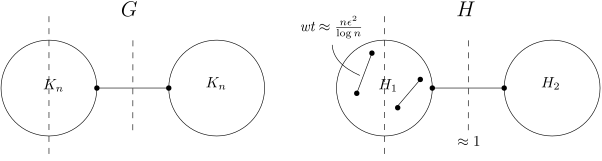
\includegraphics[scale=0.5]{images/dumbbell.svg}
\end{figure}

In the above example, $G$ is the (unweighted) dumbbell graph, two cliques
connected by a single edge. Note that $G$ is dense; $|E_G| \in \Theta(n^2)$.
Any graph $H \approx_\eps G$ for which $E_H \subseteq E_G$ must have an edge
between the two special vertices, with weight approximately 1. This is because,
as noted before, any cut of $H$ must have approximately the same weight as the
corresponding cut in $G$. By similar reasoning, we can see that the two
subgraphs $H_1$ and $H_2$ of $H$ should more-or-less behave as $\eps$-spectral
expanders so as to mimic the structure of the corresponding subgraphs in $G$,
each a copy of $K_n$. If we wish for $H$ to be sparse and still have $H
\approx_\eps G$ w.h.p., then in our randomized construction we must sample the
edges of $K_n$ each with very low probability, and scale the sampled edges'
weights at approximately $\frac{n \eps^2}{\log n}$, as in $\textsc{Expander2}$.

All this is to say that depending on the graph $G$, certain edges (e.g.\ the
``special edge'' connecting the cliques) must be sampled with higher
probability; intuitively this is because they are more important to the
structure of the graph. This suggests the idea of assigning ``importance
socres'' to edges, and sampling them with probability proporional to their
importance. We will also have to scale down the weights of the sampled edges by
their importance scores so that, in expectation, we output the original graph
$G$. This approach is due to Spielman and Srivastava \cite{SpielmanS08},
journal version \cite{SpielmanS11}. For a detailed treatment of spectral sparsifiers,
see \cite{SpielmanT08}. (See also the versions on arXiv.)

\section{Sparsifier Algorithm}

\vspace*{-\baselineskip}
\begin{algorithm}
\caption*{$\textsc{Sparsifier}(G,\eps)$:}
\begin{algorithmic}
\State Construct a probabililty distribution $\{p_e\}_{e\in E_G}$
    over the edges of $G$, \\
    edge probabilities proportional to ``importance scores'' (defined later)
\smallskip
\State\FOR{$i \gets 1,\dots,t = \Theta(\frac{1}{\eps^2} n \log n)$}
\Indent
    \vspace*{-0.2em}
    \State Sample an independent edge $e$ from $\{p_e\}$
    \State Scale it by $w_e' := \frac{w_e}{t \, p_e}$
    \State Add it to $H$
\EndIndent
\smallskip
\end{algorithmic}
\end{algorithm}

We use the notation $e_i$ to mean the $i^{\textit{th}}$ edge sampled, a random
variable. Our first observation is that the expected output of the algorithm is
the original graph. \[\E \V{L}_H = \E\brac{\sum_{i=1}^t w_{e_i}'\V{L}_{e_i}} =
t \cdot \E[w_{e_1}' \V{L}_{e_1}] = t \sum_{e \in E_G} p_e w_e' \V{L}_e =
\sum_{e \in E_G} w_e \V{L}_e = \V{L}_G,\] where $\V{L}_{(u,v)} = (\ones_u -
\ones_v)(\ones_u - \ones_v)^\T$. This is simply a consequence of the definition
of $w'$, and does not depend on the settings we give to $t$ or $\{p_e\}$ (as
long as $p_e > 0$, $\forall e \in E_G$).

What remains to be shown is that with high probability, \[(1-\eps) \V{L}_G \LE \V{L}_H
\LE (1+\eps) \V{L}_G.\] We will derive settings of $t$ and $\{p_e\}$ that suffice,
but in the meantime notice that we have a useful tool for proving statements
such as the above: matrix Chernoff bounds, of the form \[(1-\eps)\mm\bb{I} \LE
\sum \V{X}_i \LE (1+\eps)\mM\bb{I}.\] Unfortunately however, it is not enough to
apply Theorem \ref{thm:chernoff} to the samples $\V{X}_i = w_{e_i}'\V{L}_{e_i}$.

First we must normalize our samples by the pseudoinverse of $\V{L}_G$ --- if
$\psi_1,\dots,\psi_n$ are orthonormal eigenvectors of $\V{L}_G$ with corresponding
eigenvalues $\lambda_1 \le \dots \le \lambda_n$, then this is the matrix
\[\V{L}_G^+ := \sum_{i \,:\, \lambda_i > 0} \frac{1}{\lambda_i} \psi_i \psi_i^\T =
\sum_{i=2}^n \frac{1}{\lambda_i} \psi_i \psi_i^\T,\] if we assume that $G$ is
connected. Consider the matrix \[\V{L}_G^\phalf := (\V{L}_G^+)^\half = \sum_{i=2}^n
\frac{1}{\sqrt{\lambda_i}} \psi_i \psi_i^\T\] and, noting that it has the same
kernel as $\V{L}_G$ and $\V{L}_H$, symmetrically multiply the statement of $\V{L}_H
\approx_\eps \V{L}_G$ by it:
\begin{align*}
(1-\eps) \V{L}_G \LE & \V{L}_H \LE (1+\eps) \V{L}_G \\
\Longleftrightarrow
(1-\eps) \Pi \LE \V{L}_G^\phalf & \V{L}_H \V{L}_G^\phalf \LE (1+\eps) \Pi,
\end{align*}
where $\Pi := \V{L}_G^\phalf \V{L}_G \V{L}_G^\phalf = \sum_{i=2}^n \psi_i \psi_i^\T =
\bb{I} - \psi_1 \psi_1^\T = \bb{I} - \frac{1}{n}\ones\ones^\T$ is the matrix that
performs projection onto the subspace orthogonal to the kernel of $\V{L}_G$.

Now, to get a statement of the form $(1-\eps)\bb{I} \LE \sum \V{X}_i \LE
(1+\eps)\bb{I}$, we pad each of our $t$ samples by
$\frac{1}{t}\frac{1}{n}\ones\ones^T$, to fill in the kernel of $\Pi$.
\begin{align*}
\V{X}_i &:= w_{e_i}' \V{L}_G^\phalf \V{L}_{e_i} \V{L}_G^\phalf +
    \frac{1}{t}\frac{1}{n}\ones\ones^T \\
\sum_{i=1}^t \V{X}_i &= \V{L}_G^\phalf \V{L}_H \V{L}_G^\phalf + \frac{1}{n}\ones\ones^\T \\
\E \sum \V{X}_i &= \bb{I}
\end{align*}
Noting that the samples are PSD, we can apply Chernoff to $\sum \V{X}_i$ with $\mm
= \mM = 1$ to get \[\pr[(1-\eps)\bb{I} \LE \sum \V{X}_i \LE (1+\eps)\bb{I}] \ge 1 -
2n \exp(\frac{-\eps^2}{3R}).\] It remains to define the distribution $\{p_e\}$,
and to show that the samples are small in spectral norm. Our bound on the size
of the samples, $R$, will depend on $t$, and it turns out that taking $t =
\Theta(\frac{1}{\eps^2} n \log n)$ will suffice for the above Chernoff bound to
hold with high probability.

We introduce the notion of spectral norm of a matrix,
\[\norm{\V{A}} := \max_{\V{x} \ne \mathbf{0}}
\frac{\norm{\V{A}\V{x}}}{\norm{\V{x}}},\] and note that
for symmetric $\V{A} \GE 0$, \[\norm{\V{A}} = \lM(\V{A}).\]
With this notation we can write
\[R = \max_i \max_{e_i \overset{\$}{\gets} \{p_e\}} \norm{\V{X}_i}
= \max_{e_1 \overset{\$}{\gets} \{p_e\}} \norm{\V{X}_1}\]
(where the second $\max$ is over all choices of randomness),
to represent the tightest bound for which \[ \forall i
\,:\, 0 \LE \V{X}_i \LE R\,\bb{I}.\] That is,
\begin{align*}
R &:= \max_{e\in E_G} \norm{w_e' \V{L}_G^\phalf \V{L}_e \V{L}_G^\phalf
    + \frac{1}{t}\frac{1}{n}\ones\ones^\T } \\
&\ge \max \left\{ \left( \max_{e\in E_G} w_e'
    \norm{\V{L}_G^\phalf \V{L}_e \V{L}_G^\phalf} \right),
    \frac{1}{t} \norm{\frac{1}{n}\ones\ones^\T} \right\} \\
&\ge \max_{e\in E_G} \frac{w_e}{t\,p_e}
    \norm{\V{L}_G^\phalf \V{L}_e \V{L}_G^\phalf}
\end{align*}
since $\ones$ is in the kernel of $\V{L}_G^\phalf \V{L}_e \V{L}_G^\phalf$,
and therefore, $\forall e \in E_G$,
\[ p_e \ge \frac{w_e}{tR} \norm{\V{L}_G^\phalf \V{L}_e \V{L}_G^\phalf}. \]
Let us set
\[ p_e = \frac{w_e}{tR} \norm{\V{L}_G^\phalf \V{L}_e \V{L}_G^\phalf}, \]
and note that we wish to have $\sum_e p_e = 1$. This is equivalent to
\begin{align*}
tR &= \sum_e w_e \lM\paren{\V{L}_G^\phalf \V{L}_e \V{L}_G^\phalf} \\
&= \sum_{e=(u,v)} w_e \lM\paren{\V{L}_G^\phalf
    (\ones_u - \ones_v)(\ones_u - \ones_v)^\T \V{L}_G^\phalf} \\
&= \sum_e w_e \tr{\V{L}_G^\phalf
    (\ones_u - \ones_v)(\ones_u - \ones_v)^\T \V{L}_G^\phalf}
    \text{ ~ (since the matrix is rank 1)} \\
&= \tr{\V{L}_G^\phalf (\sum_e w_e \V{L}_e) \V{L}_G^\phalf} \\
&= \tr{\V{L}_G^\phalf \V{L}_G \V{L}_G^\phalf} \\
&= \tr{\Pi} = n - 1.
\end{align*}
Therefore we define the distribution $\{p_e\}$ as, $\forall e$,
\[ p_e := \frac{1}{n-1} \, w_e \norm{\V{L}_G^\phalf \V{L}_e \V{L}_G^\phalf}. \]
Picking $t := \frac{6}{\eps^2}(n-1)\log n$ gives us
\[ \pr[(1-\eps)\bb{I} \LE \sum \V{X}_i \LE (1+\eps) \bb{I}] \ge 1 - \frac{2}{n}. \]
Thus with probability at least $1 - \frac{2}{n}$,
\[ (1-\eps) \bb{I} \LE \V{L}_G^\phalf \V{L}_H \V{L}_G^\phalf
    + \frac{1}{n} \ones\ones^\T \LE (1+\eps) \bb{I}. \]
Multiplying through symmetrically by $\V{L}_G^\half$, we get
\begin{align*}
(1-\eps) \V{L}_G \LE &\V{L}_H \LE (1+\eps) \V{L}_G.
\end{align*}
That is, $H$ is an $\eps$-spectral sparsifier of $G$.

\begin{theorem}
\label{thm:sparsifier}
For any $G$, and any $0 < \eps < 1$, the graph $H$ produced by
$\textsc{Sparsifier}(G,\eps)$ is an $\eps$-spectral sparsifier of $G$.
\end{theorem}

\subsection{An aside about probabilities / leverage scores}

The scalars we used to define the probabilities $\{p_e\}$ have other
applications as well, and have a special connection to electrical networks.
\begin{align*}
&w_e \norm{\V{L}_G^\phalf \V{L}_e \V{L}_G^\phalf} \\
&= w_e \tr{\V{L}_G^\phalf \V{L}_e \V{L}_G^\phalf}
    \text{ ~ (since the matrix is rank 1)} \\
&= w_e \tr{\V{L}_G^\phalf (\ones_u - \ones_v)(\ones_u - \ones_v)^\T \V{L}_G^\phalf} \\
&= w_e \tr{(\ones_u - \ones_v)^\T \V{L}_G^+ (\ones_u - \ones_v)}
    \text{ ~ (since trace is cyclic)} \\
&= w_e (\ones_u - \ones_v)^\T \V{L}_G^+ (\ones_u - \ones_v) \\
&= w_e \Reff(u,v),
\end{align*}
where as seen in a previous lecture, $\V{L}_G^+(\ones_u - \ones_v)$ is a vector of
voltages and $\Reff(u,v) := (\ones_u - \ones_v)^\T \V{L}_G^+ (\ones_u - \ones_v)$ is
the potential difference between $u$ and $v$, if we were to send 1 unit of
current from $u$ to $v$.

The quantity $w_e \Reff(e)$ is often called the leverage score of edge $e$:
\[ \textit{Lev-score}(e) := w_e \Reff(e). \]

\subsection{Motivation for the next lecture}

It is worth noting that a na\"ive, exact computation of $\V{L}_G^+$ would take time
$O(n^3)$, and thus calculating the probabilities $\{p_e\}$ would take time
$O(n^3 + m) = O(n^3)$. This is often infeasible in practice, and we will see
next lecture that we can bypass this $O(n^3)$ computation by instead computing
approximate solutions to $L x = b$.

\bibliographystyle{plain}
\bibliography{papers}

\end{document}

%%% Local Variables:
%%% mode: latex
%%% TeX-master: t
%%% End:
